\Chapter{Interaktív grafikus elemek}

\Section{Widget-ek}

A program használata során a felhasználó különféle virtuális interaktív grafikus elemekkel léphet kapcsolatba, segítségükkel irányíthatja a programot, befolyásolhatja a prezentáció menetét. Az elemek más-más funkcióval rendelkeznek. Megjelenítés szempontjából minden grafikus elem képek segítségével jelenik meg. A következőkben néhány lehetséges widgetet kívánok definiálni, melyek segítségével...

\begin{itemize}
	\item \textbf{Button}: Az egyik legegyszerűbb interaktív elem, egy virtuális nyomógomb, melyet megnyomva egy meghatározott funkciót érhetünk el.
	\item \textbf{Grabbable}: A prezentáló személy a \textit{Drag and Drop} gesztus-sorozat segítségével megtudja fogni az ilyen tulajdonsággal rendelkező elemeket, majd kívánt új pozíciójába helyezheti azt.
	\item \textbf{Shiftable}: A felhasználó \textit{Shift} gesztus segítségével léphet kapcsolatba az ilyen típusú elemekkel, a képtartományon belül tologathatja azokat.
	\item \textbf{Openable}: Ezen elemek nyithatóak, zárhatóak.
	\item \textbf{Rollable}: Egy rögzített ablakon keresztül vizsgálhatunk egy hosszú kép részletét. A felhasználónak lehetősége van megváltoztatnia a megjelenítendő képrészletet a virtuális elem görgetésével.
	\item \textbf{Tuner}: Virtuális "potméter". A \textit{Rotation} gesztussal léphetünk kapcsolatba vele és értékeket állíthatunk be egy meghatározott tartományon.
\end{itemize}

\Section{Képek hozzáadása a videófolyamhoz}

A programban elérhető interaktív grafikus elemek mindegyike képek segítségével jelenik meg. A videófolyam képkockáira az úgynevezett \textit{Alpha blending} technikával helyzehetünk el átlátszóság értékkel képeket. A módszerhez két képre van szükségünk. Esetünkben ezen képek a videófolyam aktuális képkockája és az adott widget képe lesz. Mivel az eljárás egy mátrixművelet, ezért a képeknek hasonló tulajdonságokkal kell rendelkezniük. Egyeznie kell a felbontásnak, és a csatornák számának is. A megjelenítendő widgetek a videófolyam felbontásától különbözni fognak, ezért a videófolyam egy kiragadott képrészletét kell használnunk, hogy a felbontásra vonatkozó megkötés is teljesüljön.

Két esetet különíthetünk el. Az első esetben azt az esetet(?) nézzük, amikor mindkét kép három csatornával rendelkezik, vagyis a három alapszínek intenzitásértékeit tartalmazzák. Ebben az esetben az \textit{Alpha blending} technika segítségével az egyes képek átlátszóságát állíthatjuk. Ha nem szeretnénk ilyen hatást elérni, akkor egyszerűen csak kicserélhetnénk a videófolyam widget területére eső pixeleit a widget pixeleire. De a program kezelése szempontjából indokolt egy kis átlátszóság alkalmazása, hogy a prezentáló személy lássa, hogy a widget mögött mi helyezkedik el.

A módszerhez definiálnunk kell az $\alpha$, $\beta$ és súlyokat és a $\gamma$ értékét.
\begin{align*}
	\text{kimenet}_{x,y} = \alpha \cdot \text{kép1}_{x,y} + \beta \cdot \text{kép2}_{x,y} + \gamma
\end{align*}
Ha $0<\alpha<1$ és $\beta = 1 - \alpha$ és $\gamma = 0$, akkor a \textit{sztenderd alpha blend egyenletet}\cite{bradski2008learning} kapjuk:
\begin{align*}
		\text{kimenet}_{x,y} = \alpha \cdot \text{kép1}_{x,y} + (1-\alpha) \cdot \text{kép2}_{x,y}
\end{align*}
Az $\alpha$ súly helyes megválasztásával módosíthatuk a cél képre helyezendő kép átlátszóságánal mértékét.

A második esetben olyan képeket szeretnénk illeszteni, az általánosan háromcsatornás videófolyamra, melyek $\alpha$ csatornával is rendelkeznek, azaz egy egyes pixelek átlátszóságáról is hordoznak információkat. A legelterjettebb ilyen tulajdonsággal rendelkező képformátum a PNG (\textit{Portable Network Graphics}). Hogy az ilyen típusú képeket az \textit{Alpha blending} elvégzéhez előtt a következőképpen kell feldolgoznunk:\\
Jelöljük a háttérképet $\boldsymbol H$-val, a ráillesztendő 4 csatornás képet pedig $\boldsymbol E$-vel. Feltételezzük, hogy az intenzitásértékek 0 és 255 közötti tartományon vehetnek fel értékeket.
\begin{figure}[h]
	\centering
	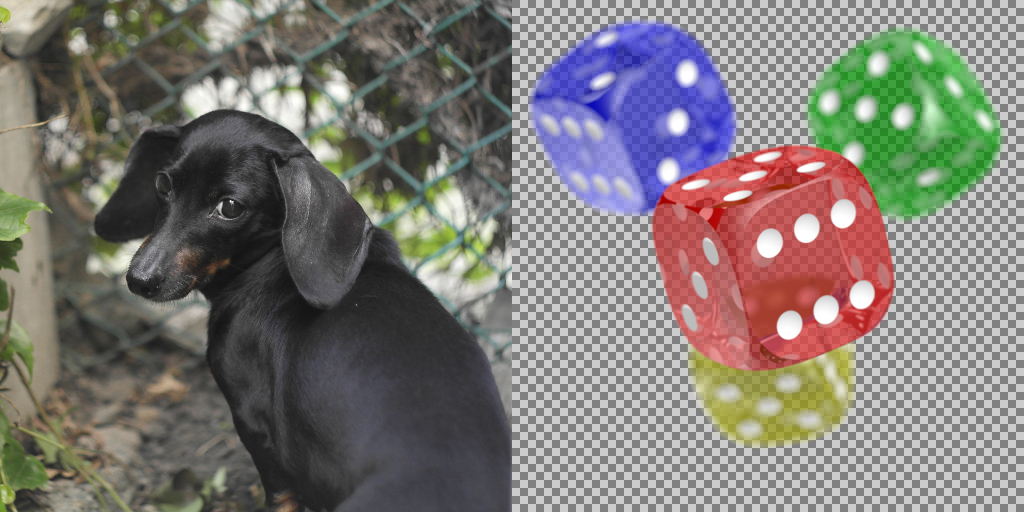
\includegraphics[width=6.82truecm, height=3.41truecm]{images/blending_01.png}
	\caption{Az eredeti képek ($\boldsymbol H$ és  $\boldsymbol E$)}
	\label{fig:blend01}
\end{figure}	
\begin{enumerate}
	\item Vegyük az $\boldsymbol E$ képet és válaszuk két felé: $\boldsymbol E_{sz}$ (szín) és $\boldsymbol E_\alpha$ ($\alpha$) csatornákra.
	\item Határozzuk meg a $\boldsymbol E_{\alpha H}$ háttérmaszkot az $\boldsymbol E_\alpha$ inverzével.
		\begin{align*}
			\boldsymbol E_{\alpha H} = 255 - \boldsymbol E_\alpha
		\end{align*}
		\begin{figure}[h]
			\centering
			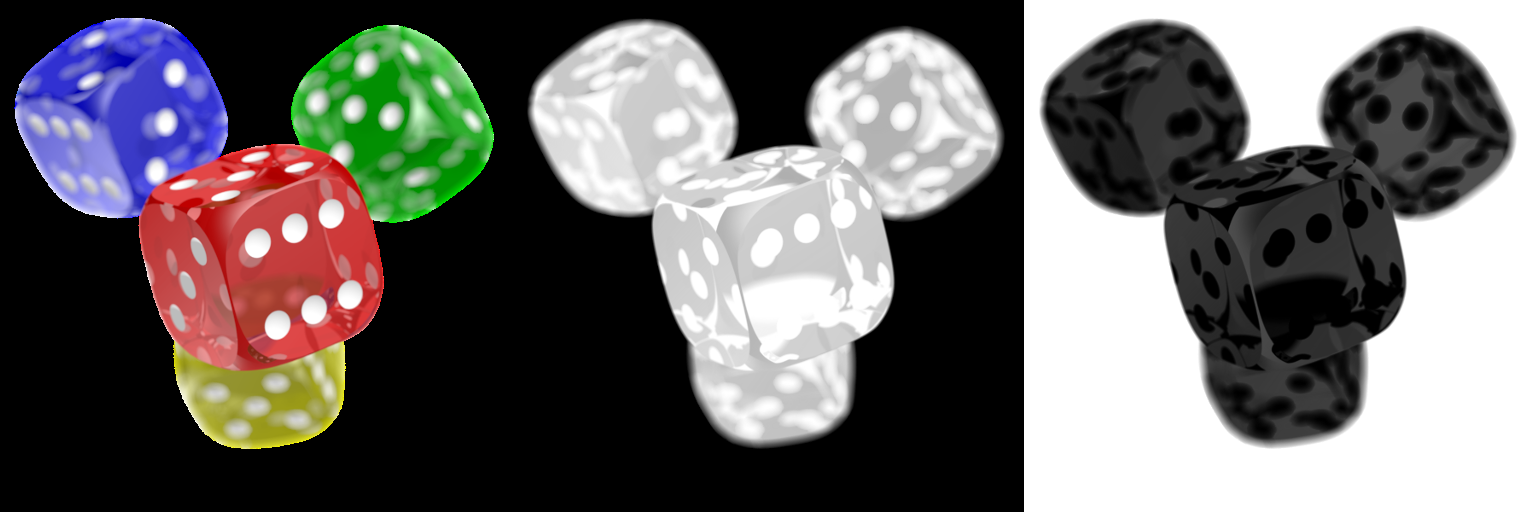
\includegraphics[width=10.24truecm, height=3.41truecm]{images/blending_02.png}
			\caption{$\boldsymbol E_{sz}$, $\boldsymbol E_\alpha$, $\boldsymbol E_{\alpha H}$}
			\label{fig:blend02}
		\end{figure}	
	\item Alakítsuk át a $\boldsymbol E_{\alpha H}$ háttérmaszkot és az eredeti $\boldsymbol E_\alpha$ maszkot háromcsatornássá, hogy a következő számításokat el tudjuk végezni.
	\item Számoljuk ki az összemosandó képeket a maszkok segítségével. Itt áttérünk 0 és 1 közötti intenzitásértékekre.
		\begin{align*}
				\boldsymbol H_m &= \left(\frac{\boldsymbol H}{255}\right) \cdot \left(\frac{\boldsymbol E_{\alpha H}}{255}\right)\\
				\boldsymbol E_m &= \left(\frac{\boldsymbol E}{255}\right) \cdot \left(\frac{\boldsymbol E_\alpha}{255}\right)
		\end{align*}
\end{enumerate}
Az \textit{Alpha blendig}-et pedig ebben az esetben a következőképpen hajtjuk végre:
\begin{align*}
	\text{kimenet} = 255 \cdot \boldsymbol H_m + 255 \cdot \boldsymbol E_m
\end{align*}
\begin{figure}[h]
	\centering
	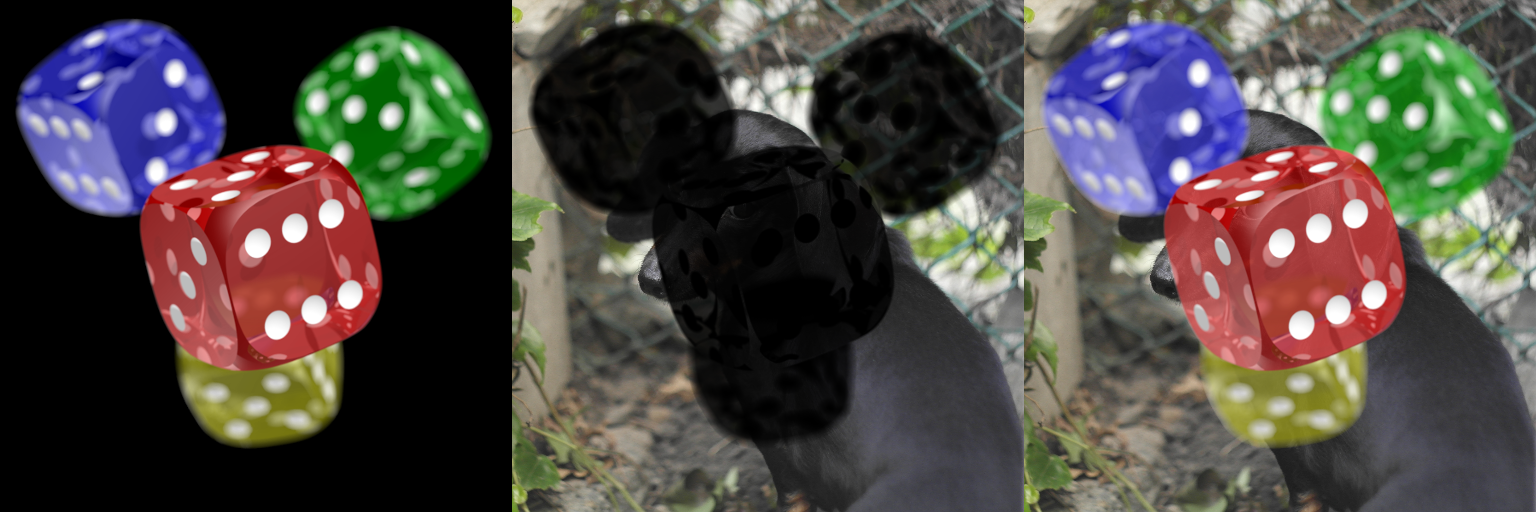
\includegraphics[width=10.24truecm, height=3.41truecm]{images/blending_03.png}
	\caption{$\boldsymbol E_m$, $\boldsymbol H_m$ és a kimeneti kép}
	\label{fig:blend02}
\end{figure}	
		
% Forrás??? Stackoverflow
% https://stackoverflow.com/questions/36921496/how-to-join-png-with-alpha-transparency-in-a-frame-in-realtime/37198079#37198079

% Képeken keresztül szemléltetni, hogy mi is történik!!!

\Section{Widgetek tulajdonságai}

\SubSection{Button}

A \textit{Button} vagy \textit{Nyomógomb} működtetése rendkívül egyszerű. Aktiválásához a felhasználónak egyszerűen csak a gomb területére kell emelnie például a kézfejét, a gomb pedig egy bizonyos idő elteltével reagál.

A gombon belüli mozgás figyelésére segítségül hívhatjuk a \textit{Hőtérkép} csoportjait. Ha egy csoport súlypontja a gombon belül helyezkedik el, majd ha megszűnik (vagyis ha a csoporthoz tartozó valódi objektum abbahagyja a mozgását), akkor a megszűnt csoport súlypontjának a koordinátáira egy figyelendő pontot helyezünk. Ha a vizsgálandó pont kilép a gomb tartományából egy előre meghatározott időn belül, akkor nem történik semmi. Ha viszont a vizsgálandó pont a gomb területén belül marad, a gomb aktiválódik. 
Vagyis ez egy valós helyzetben a következőképpen nézhet ki: A felhasználó a gomb területére irányítja a kézfejét, a kézfejének apró mozdulatai (melyek nem figyelhetőek meg a \textit{Hőtérképen} a képzaj kiküszöbölése miatt) egy vizsgálandó pont segítségével lesznek követve, amely a már ismert \textit{Optical-Flow} technikával valósul meg.

A véletlen gombnyomás, nem kívánt viselkedés elkerülése érdekében időkeretet kell megszabnunk a vizsgálandó pont a gombon belül töltött idejére. Ezen időintervallumnak viszonylag rövidnek kell lennie, hogy a felhasználói élmény ne romoljon (ne kelljen várni túl sokáig a gombnyomásra), viszont nem lehet túl rövid ahhoz, hogy egy esetleges véletlen mozdulat aktiválni tudja. A helyes időkeret megválasztása a gomb méretétől is függhet. Tapasztalati adatok szerint 0.2-0.5 másodperc közötti időkeret használata megfelelőnek tűnik.

\SubSection{Grabbable}

A megfogható tulajdonsággal rendelkező objektumokat a felhasználó a képtartományon belül szabadon áthelyezheti kedve szerint. A művelethez egy \textit{Drag and Drop} gesztust-sorozatot kell végrehajtania. A \textit{Blink} gesztus kiadásakor minden esetben számolódik egy pozíció érték, amely a kézfej helyzetét kívánja megbecsülni. Ha ezen pont az elem területére esik, akkor a pontot innentől kezdve vizsgálandó pontnak kell tekintenünk. A pont helyzetének frissítése az \textit{Optical-Flow} technikával történik. Az elem új pozíciója a ponthoz képest módosul, vagyis az elem a felhasználó kézfejét követi.
Amint elnavigálta a kívánt pozícióba az új elemet a felhasználó, eg újabb \textit{Blink} gesztussal a helyére teheti azt.

Hogy az elem véletlenül se lépjen ki a videófolyamból, korlátoznunk kell a lehetséges mozgásterét a képtartományra. Vagyis az elem szélei nem mehetnek túl a kép szélein. Ezen megszorítás a többi elemre is vonatkozik.

\SubSection{Shiftable}

A tologatható elemekkel \textit{Shift} gesztus segítségével léphetünk kapcsolatba. Az irányukba történő mozgásra megeggyező irányú mozgással reagálnak. Működésére olyan hatás jellemző, mintha az elemet tologatnánk.

\SubSection{Openable}

Ezen virtuális elemek megjelenés szempontjából hasonlítanak egy pargamen tekercshez, belső tartalmuk kezdetben rejtett, azonban a felhasználónak lehetősége van kinyitni, megmutatva a belső tartalmát, majd becsukni az adott elemet.

A \textit{Tologatható elemekhez} hasonlóan, \textit{Shift} gesztussal léphetünk kapcsolatba az ilyen tulajdonságokkal ellátott elemekkel, viszont az ilyen típusú elemek mozgása egy bizonyos tengelyre korlátozódik, kezdőpozícióját megtartja és a megjelenítendő képrészlet nagysága változik csupán. Az elemhez definiálnunk kell a \textit{header} szekció méretét, ami az elem minimum méretét fogja megadni. Mivel az elem viselkedését a vektormező adataiból számoljuk, ezért a \textit{header} mérete nem lehet kisebb a rács sűrűségéből számított lépésköznél, hiszen ilyenkor bizonyos esetekben az elem becsukott állapotban egyetlen kontrollpontot sem fedne le, így a felhasználó nem tudna interakcióba lépni vele.
Az elem tényleges mérete pedig a teljesen kinyitott állapototára vonatkozik.

\SubSection{Rollable}

A \textit{Rollable} virtuális elemek rögzített pozíciójú, fix méretű widgetek.

Működés szempontjából hasonlítanak egy diavetítőre, hiszen a hozzá tartozó nagy méretű képet egy ablakon keresztül szemlélhetjük, a megjelenítendő képrészletet pedig a felhasználó kedve szerint változtathatja, vagyis úgy tűnik, mintha görgetné az adott ablakon található tartalmat.

Az ilyen típusú widgeteket is a \textit{Shift} gesztus segítségével vezérelhetjük. A gesztus végrehajtása során kiszámolódik a megjelenítendő képrészlet \textit{kezdőpozíciója}, ami alapján, az \textit{ablak méretét} figyelembe véve meghatározható az eredeti képből kivágandó képrészlet.
A helyes működés érdekében a képrészlet kezdőpozíciójának értékét korlátoznunk kell. Az értéke nem lehet nullánál kisebb, illetve nem lehet nagyobb a hozzá tartozó kép magasságának és az ablakméret magasságának különbségénél ($y$ tengelyen görgethető \textit{Rollable} widget esetében).
\begin{align*}
	0 \leq \textit{képrészlet kezdőpozíciója} \leq (\textit{képmagasság} - \textit{ablakmagasság})
\end{align*}

Így elkerülhetők a hibás vágások, illetve megakadályozható a kép kicsúszása az ablakból.
A megjelenítendő kép

\SubSection{Tuner}

A \textit{Tuner} widget-et működése és megjelenése szempontjából egy potméter gombnak képzelhetjük el. Segítségével a felhasználó különböző értékeket állíthat be.
Az ilyen típisú widgeteket a \textit{Rotation} gesztus segítségével érhetjük el. Ha a \textit{Rotation} becsült forgási középpontja az adott elem belsejébe esik, az aktiválódik és a gesztus feldolgozása során további információkat figyelembe véve változik meg az állapota.

A felhasználó definiálhatja, hogy az egyes ilyen típusú widget-ek értékei milyen tartományon szerepelhetnek, vagyis meg kell határoznia a legkisebb és legnagyobb értéket, amelyet a widget felvehet. Az értékek számítása a forgási szög függvényében történik. A widget élete során kapott elfordulás szögei szummázódnak és a widget értéke ezen szummázott szög alapján számolódik. A szummázott összegre vonatkozik egy olyan megszorítás, hogy értéke, fokokban nézve, nem lehet 0$^{\circ}$ alatt és 360$^{\circ}$ fölött. Egy tomptó értéket is be kell vezetnünk, amellyel a szummázás előtt az eredeti szög értékét csökkentjük. Ez az érték tapasztalata alapokon 10, vagyis a tényleges becsült forgási szög tizedét vesszük csak figyelembe a finomabb működés érdekében.
Megjelenés szempontjából a \textit{Tuner} widget valóban elfordul. A hatás eléréséhez minden iterációban a widget súlypontját és a szummázott szöget felhasználva affin transzormációval elforgatjuk a widget eredeti képét.
